%
%  jsag
%
%  Created by franzi on 2013-03-24.
%  Copyright (c) 2013 __MyCompanyName__. All rights reserved.
%
\documentclass[twocolumn]{article}

% Use utf-8 encoding for foreign characters
\usepackage[utf8]{inputenc}

% Setup for fullpage use
\usepackage{fullpage, hyperref}

\usepackage{abstract}
% Uncomment some of the following if you use the features
%
% Running Headers and footers
%\usepackage{fancyhdr}

% Multipart figures
%\usepackage{subfigure}

% More symbols
%\usepackage{amsmath}
%\usepackage{amssymb}
%\usepackage{latexsym}

% Surround parts of graphics with box
\usepackage{boxedminipage}

% Package for including code in the document
\usepackage{listings}

% If you want to generate a toc for each chapter (use with book)
\usepackage{minitoc}

% This is now the recommended way for checking for PDFLaTeX:
\usepackage{ifpdf}

%\newif\ifpdf
%\ifx\pdfoutput\undefined
%\pdffalse % we are not running PDFLaTeX
%\else
%\pdfoutput=1 % we are running PDFLaTeX
%\pdftrue
%\fi

\ifpdf
\usepackage[pdftex]{graphicx}
\else
\usepackage{graphicx}
\fi

\def\M2{{\it Macaulay2}}

\title{A Web Application for Macaulay2}
\author{Lars Kastner\\ Freie Universit\"at Berlin \\{\small kastner\char`\@math.fu-berlin.de} \and
Franziska Hinkelmann\\TNG Technology Consulting GmbH \\{\small franziska.hinkelmann\char`\@tngtech.com} \and 
Michael Stillman\\Cornell University \\{\small mike\char`\@math.cornell.edu} \thanks{Stillman has been supported by NSF grants DMS 08-10909 and 10-02210. Hinkelmann has been supported by NSF award 0635561. Kastner by DFG SPP 1489. 
} }


\date{}

\begin{document}



\ifpdf
\DeclareGraphicsExtensions{.pdf, .jpg, .tif}
\else
\DeclareGraphicsExtensions{.eps, .jpg}
\fi


\twocolumn[
    \maketitle
        \begin{onecolabstract}
            \M2 is a software system devoted to supporting research in algebraic
            geometry and commutative algebra, whose creation has been funded by the
            National Science Foundation since 1992. It is a command-line tool that
            has no graphical user
            interface. 
            This manuscript describes a new web application for \M2. It requires no installation
            and provides a graphical user interface. Therefore making \M2 more 
            accessible, especially to first time users and students. 
            The web application has all features that the desktop version offers. 
            In addition, it contains tutorials
            that explain different concepts of algebraic geometry such as
            Gr\"obner bases. Users can also create their own tutorials.
            The web version has been used in courses at Cornell
            University, Harvard University, Georgia Tech, and Free University of Berlin.
        \end{onecolabstract}
]
\saythanks
\section{Introduction}

\M2 is a software system devoted to supporting research
in algebraic geometry and commutative algebra, whose creation and
development have been funded by the National Science Foundation
since 1992~\cite{M2}. We developed a web version of \M2. It is available at \cite{webM2}.
The web version has the advantage that users do not need to
download or install any software. A browser and internet connection are enough to
run calculations in \M2. It
has the same functionality as the desktop version,
albeit users might have access to less resources
than on their own machine. Users can upload files,
load packages, and generate files such as images.

Our primary motivation for creating this web application was to
provide an easy to use experience for classroom and student use.
Having students download and install software such as \M2 is time
consuming and inevitably there are some situations for which this
process fails or takes significant effort to get running, e.g., on Windows.  
The web application is designed to
be able to handle many students at once. To keep it as simple as possible,
there is no sign-up or login process.


 The web version was used at the Syzygies
meeting in Berlin in May 2013, with about 70 users. It is being used in courses at Cornell
University, Harvard University, Georgia Tech, and Free University of
 Berlin. We would like to point out that the
site is suited not only for beginners, but also for seasoned experts.

We considered off the shelf solutions, such as the Sage
notebook~\cite{sagenotebook}, but decided that we wished for a more
lightweight solution, and one that did not require users to create
new accounts at a web site.  Nothing available seemed to meet our
needs, hence the current system.

The web version runs under the Chrome, Firefox and Safari web browsers, but not
under Internet Explorer.  On the iPad, it runs under Chrome and
Safari, although it seems that Chrome offers a nicer user experience.
It runs under recent versions of Android ($4.0$ and higher).

In addition to the interface to \M2, the web application provides several tutorials.  
Users can also create their own
tutorials and share them with other \M2 users.  

\begin{figure*}[htb]
    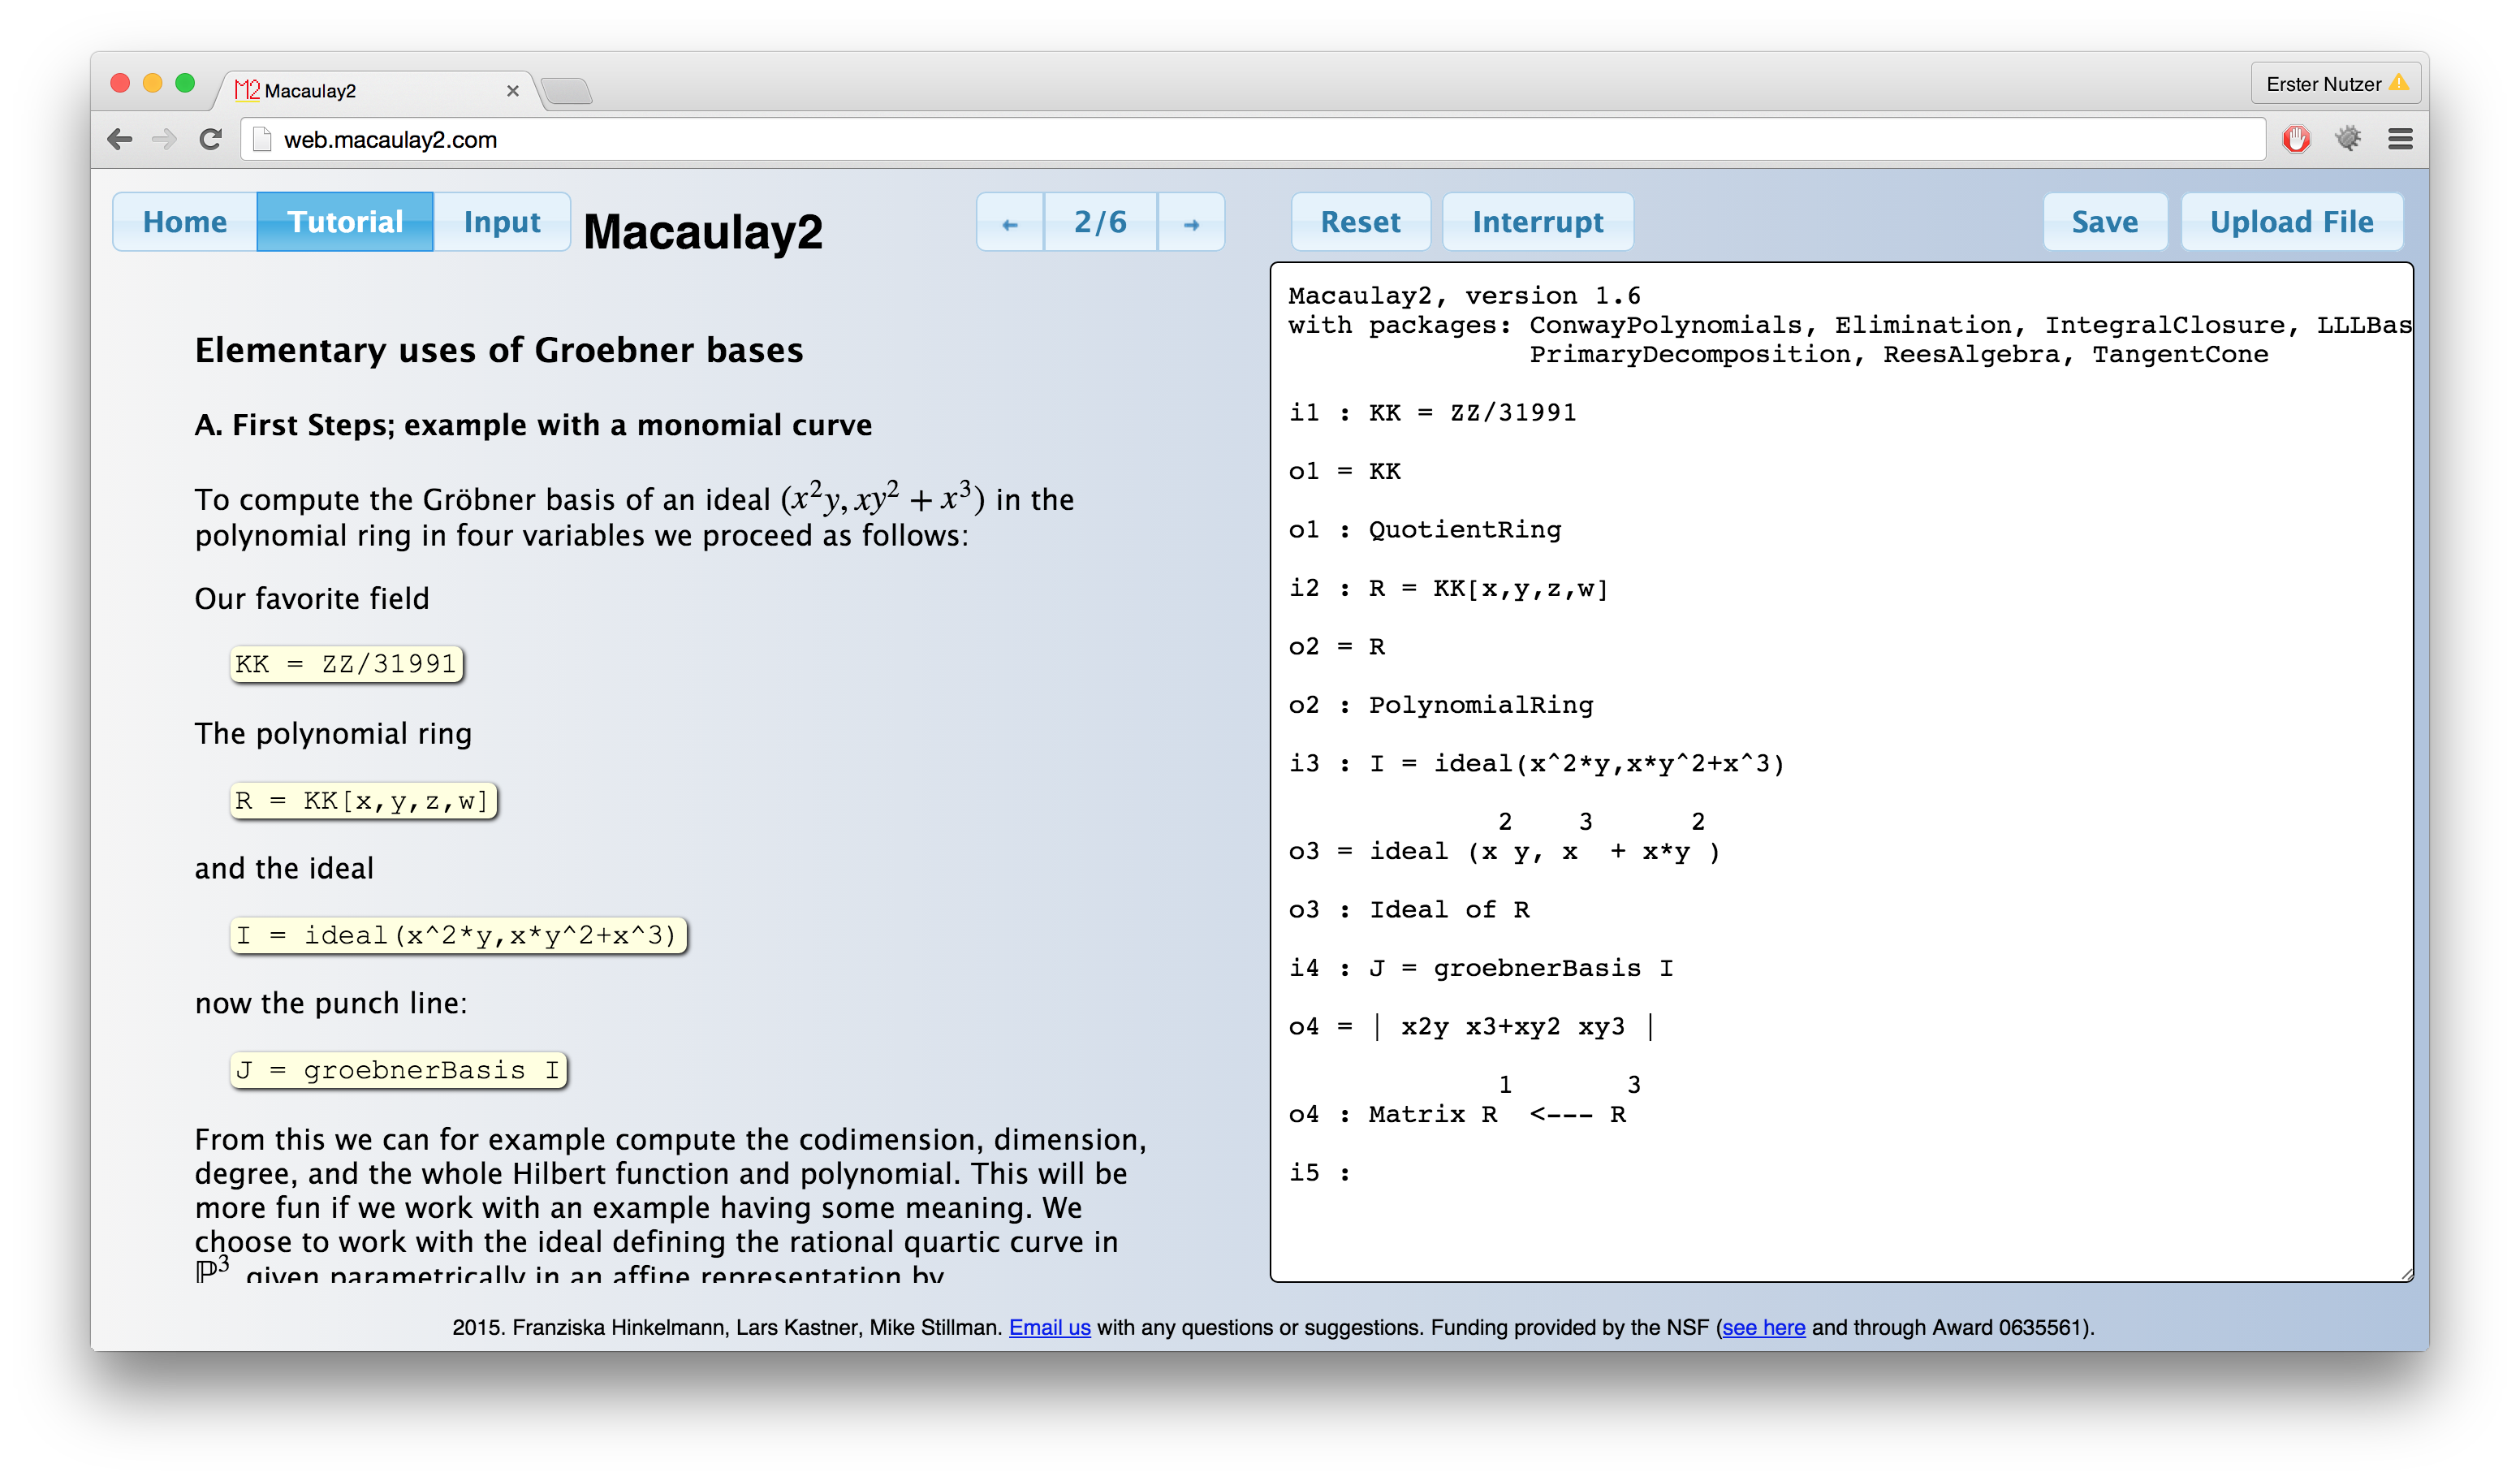
\includegraphics[width=.99\textwidth]{homeWebsite.jpg}
    \caption{A typical view in the web version of \M2. The left hand
        side shows a tutorial giving an introduction to Gr\"obner
        bases. Text in yellow can be clicked and is then executed by
        \M2 on the server. The complete output of the calculations
        is show on the right hand side. Clicking {\it Home, Tutorial, Input}
        changes the left hand view, {\it Reset, Interrupt}
        reset and interrupt the \M2 session on the server, {\it
        Save} provides both the input and the output of the current
        session to the user as a text file, and {\it Upload} uploads files
        that can then be accessed by \M2.}
\label{fig:home}
\end{figure*}


In Section 2, we describe the basics of using the web application.
Section 3 details how to create tutorials.
Providing a program such as \M2 which allows users to
access system resources presents a number of challenges to keep users
from naively or mischievously misusing the system.  In Section 4, we
provide technical details of the application.
In the last section we describe future features the web application.

The system is open source, and available on GitHub (see \cite{github}).
If you would like more information on using this in your own courses,
or if you have suggestions, please contact one of us.


\section{How to use the website}

An important
design decision is to keep the interface as simple as possible.
Therefore there is no login or registration.

The right hand side provides a shell like environment running
\M2. You can type into it and use the arrow keys for
navigating through your command history. You can use the tabulator 
key for command completion. 

On the left hand side, you can switch between {\it Home}, {\it
  Tutorial}, and {\it Input}. {\it Home} shows the available
 tutorials. {\it Tutorial} shows the currently selected
tutorial. Tutorials are interactive and contain executable pieces of
\M2 code that are run by clicking on them. {\it Input} is a
text area in which you can type \M2 commands and execute them.

All code executed, either by clicking on interactive parts in a
tutorial or by entering code in the {\it Input} window, will appear in 
the terminal on the right hand side together with the \M2 output.


The {\it Reset} button resets a \M2 session, i.e., restarts 
the \M2 process: it stops any running calculation, deletes all variables, 
unloads all packages, and then reloads the standard packages.

The {\it Interrupt} button stops a running calculation, without
resetting the \M2 session. This is useful if you want to stop a long calculation.

\subsection{Features}
You can run any command in the \M2 web application that you can run in the desktop version.
To find the current version of \M2,
enter and evaluate: {\tt version}.  You can load a package
 using {\tt loadPackage} or {\tt needsPackage}, e.g. {\tt needsPackage "BoijSoederberg"}.  
You can upload a new packages by clicking the {\it Upload file}
button. Similarly, you can upload any other file that you want to 
read or manipulate with \M2, e.g., text files with data. 

\begin{figure*}[htb]
    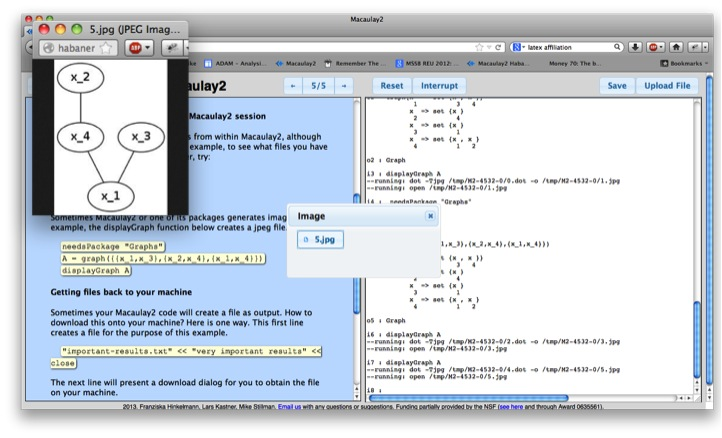
\includegraphics[width=.95\textwidth]{withGraph.jpg}
    \caption{Screenshot after the user
      generated an image. Some \M2 packages can generate
      graphs. By invoking the command {\tt displayGraph}, the image is
      generated on the server and displayed to the user.}
    \label{fig:graph}
\end{figure*}

Results from a session can be retrieved by using the {\it Save}
button, or by using copy and paste. If \M2 generates
images such as graphs, those are presented to the user, see Figure \ref{fig:graph}.


Session are usually kept alive for several days. When you start a \M2 session and visit the web app at a later time, 
you will find your previous session. Occasionally, 
we have to reboot the server or deploy a new version, this, 
unfortunately, will delete your session. Also, we have to restrict resources since you are on a shared machine.

\section{Tutorials}

You can create your own tutorials for the web version. If you teach a course,
email your tutorial to your students. They can include your tutorial in their web app by clicking
{\it Load Tutorial} on the website.
If you want to share a tutorial with the community, we would
be happy to include them on the website!

You can use the \M2 package {\it DocConverter}.
It converts a file from {\it SimpleDoc} to the tutorial specific HTML. Please see the
{\it DocConverter} package for instructions and examples.


\section{Internal structure}

We choose to implement the server in Node.js
because of Node.js's event-driven, non-blocking I/O model \cite{nodejs}.
The Node.js server functions as a bridge between \M2 instances and end users.

For every user we start a new \M2 process and
provide them with the underlying Linux system in a separate virtual environment.
This allows advanced users to
interact with the file system or run shell commands by using \M2's {\tt get} 
command:

\begin{verbatim}
i1 : -- get information on the underlying
     -- operating system
     get "!uname -mrs" 
o1 = Linux 3.13.0-49-generic x86_64

i2 : -- write to a file     
     "results.txt" << "Hello!" << close
o2 = results.txt
o2 : File

i3 : -- list all files in the current
     -- directory
     get "!ls"
o3 = results.txt

i4 : -- obtain the file
     get "!open results.txt"
\end{verbatim}

Technically, this is achieved by using Docker containers \cite{docker}. Docker implements
a high-level API to provide lightweight containers that run processes in isolation.
We start a new Docker container running \M2 for every user. The Node.js
server communicates with Docker containers via {\it ssh}. This allows us to easily
scale the application as demand grows.

To ease the setup process we provide a virtual machine that contains both the Node.js server
and Docker. This virtual machine is configured using {\tt vagrant}, a tool to create and
configure reproducible and portable development environments \cite{vagrant}.

\section{Conclusion}

By providing \M2 as a web application, we hope to lower the
 entry barrier for new users, therefore increasing the number 
 of users and fostering research in computational algebraic geometry and commutative algebra. 


We are collaborating with several mathematicians to develop more tutorials.
We plan to substantially increase the number of tutorials in the tutorial database over the next semester.


We envision some form of session sharing which allows to use the web app as a tool for collaborative research.


The application was designed with \M2 in mind, but
the entire structure will work for other command line programs such as Singular \cite{singular},
and GAP \cite{GAP4}. A similar web application for Singular is work in progress.

\section{Acknowledgments}

We would like to thank Charles Boyd, Dan Grayson, Greg Smith, and Benjamin Lorenz for
fruitful discussions on system security and on user interface design.

\bibliographystyle{plain}
\bibliography{references}
\end{document}
